\section{Data Sources}
\label{sec:data_sources}

\begin{figure}[H]
    \hspace*{-2.5cm}
    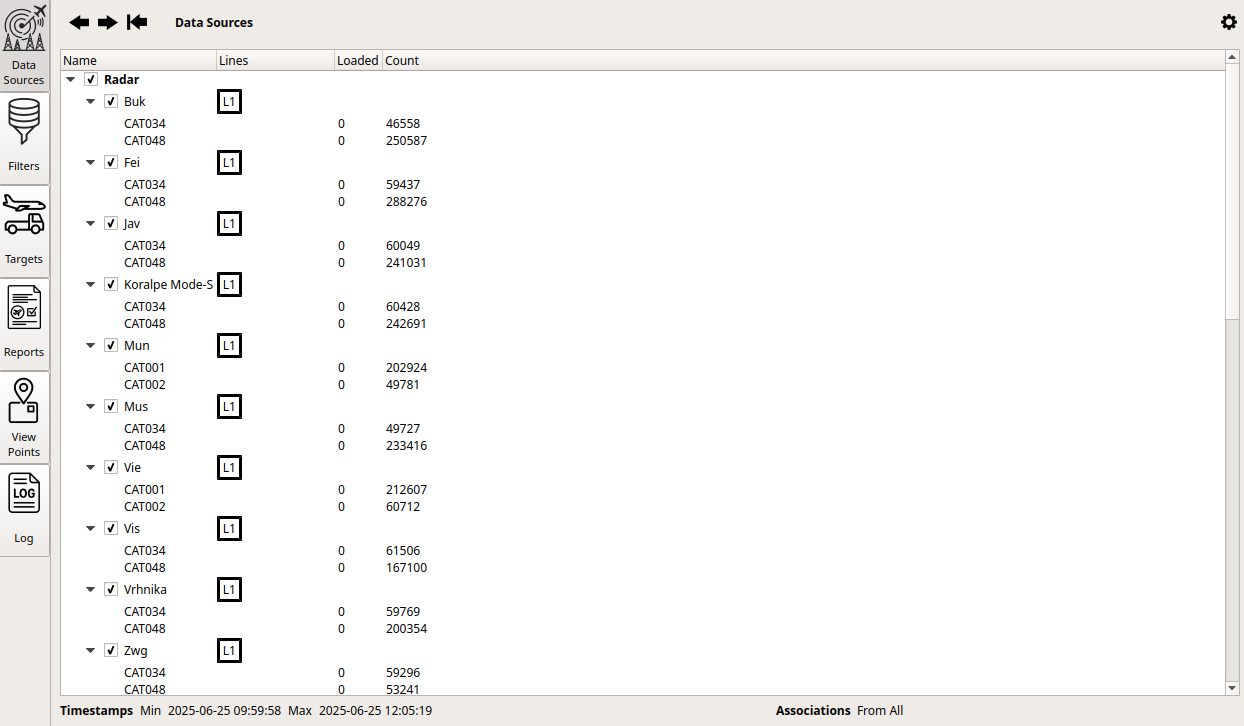
\includegraphics[width=19cm,frame]{figures/ui_data_sources.png}
  \caption{Data Sources Overview}
\end{figure}

In this Flight Deck tool, the Data Sources existing in the database are shown. 
Data sources are added to the database if data during the import process was associated with the respective Data Source (and the respective Data Source line). \\

Data Sources are grouped by DSType (Data Source Type, e.g. Radar, MLAT, ...), and can have up to 4 active lines (L1-L4). Each line for which data exists in the database is shown as a button. \\

Loading of the respective data can be changed on 3 levels:

\begin{itemize}
 \item By DSType (using checkbox)
 \item By Data Source (using checkbox)
 \item By Data Source line (using button, strong border means active)
\end{itemize}
\  \\

At the bottom, the 'Associations' label indicates if association information exists, and from which Data Source it was generated.\newline

The \includegraphics[width=0.5cm,frame]{../../data/icons/edit.png} button in the top right corner can be used to execute several actions for convenience.
Clicking the button opens the following menu.

\begin{figure}[H]
    \center
    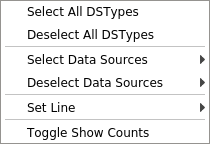
\includegraphics[width=4.5cm,frame]{figures/ui_data_source_configmenu.png}
  %\caption{Data Sources Overview}
\end{figure}

\paragraph{Select All DSTypes / Deselect All DSTypes}

Selects/deselects all listed Data Source types. The selection of individual Data Sources will remain as is.

\paragraph{Select Data Sources / Deselect Data Sources}

Can be used to conveniently select or deselect certain groups of Data Sources.

\begin{figure}[H]
    \center
    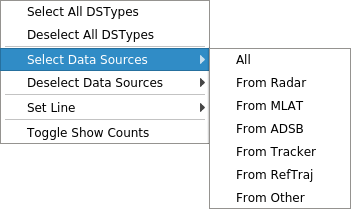
\includegraphics[width=7cm,frame]{figures/ui_data_source_configmenu_select.png}
  %\caption{Data Sources Overview}
\end{figure}

The selection can either be applied to all Data Sources ('All'), or to Data Sources of a certain Data Source type. 

\paragraph{Set Line}

Can be used to conveniently select or deselect certain Data Source lines.

\begin{figure}[H]
    \center
    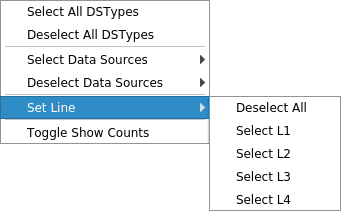
\includegraphics[width=7cm,frame]{figures/ui_data_source_configmenu_lines.png}
  %\caption{Data Sources Overview}
\end{figure}

'Deselect All' will deselect all lines. 'Select L1' to 'Select L4' can be used to select a certain Data Source line for all Data Sources.

\textbf{Note} that if the selected line is not available, all available lines will be deselected.

\paragraph{Toggle Show Counts}

Toggles the display of loaded data counts below each listed Data Source. Example:

\begin{figure}[H]
    \center
    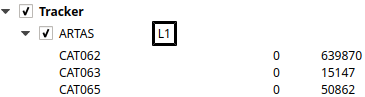
\includegraphics[width=9cm,frame]{figures/ui_data_source_configmenu_counts.png}
  %\caption{Data Sources Overview}
\end{figure}
